\section{Experiments}
\label{sec:experiments}
\paragraph{Benchmarks.}
We use LIBERO~\cite{libero} for generalization, LIBERO-Pro~\cite{liberopro} for robustness, RoboTwin~2.0~\cite{robotwin} for dual-arm manipulation, and RoboMME~\cite{robomme} for memory-dependent behavior. Five distinct real-robot tasks additionally test articulated, contact-rich, and deformable-object manipulation. LIBERO uses an overall average, LIBERO-Pro retains its five perturbation subsets, and RoboTwin reports Easy and Hard settings.

\paragraph{Baselines.}
We compare $\pi_{0.5}$, OpenVLA-OFT, VLA-$\Delta$, Physical Words, AW-0, and LexiconVLA~\cite{pi05,oft,vladelta,physicalwords,aw0,lexiconvla}. The RoboMME study compares general-purpose policies and a matched text-conditioned controller, rather than specialized memory architectures. The component and controller studies share three RoboTwin tasks: Handover Block, Place Object Basket, and Put Bottles Dustbin.

\paragraph{Report status.}
All projected scores, including comparator values, are planning estimates; the feature plot is synthetic. Published references are marked separately. Each experiment specifies its purpose and procedure, expected pattern, and conditional interpretation. Full settings and statistical tests are in Appendix~\ref{app:experiments}.

\subsection{Benchmark Performance}
\label{sec:benchmarks}
\textbf{Purpose and procedure.} We test whether reusable programs and pose grounding transfer beyond nominal training conditions. Policies use matched demonstration identities and budgets, then run on the same LIBERO, LIBERO-Pro, and RoboTwin evaluation manifests. LIBERO-Pro changes object attributes, initial positions, instruction phrasing, task goals, and environments. Nested demonstration budgets and held-out primitive compositions separately test data efficiency and reuse. Table~\ref{tab:liberopro} gives the expected benchmark scenario.

\begin{table*}[t]
\centering
\footnotesize
\setlength{\tabcolsep}{2.5pt}
\caption{\textbf{Benchmark planning estimates (\%).} All scores are projected, including baselines. LIBERO-Pro averages five perturbations. -- indicates an unplanned evaluation.}
\label{tab:liberopro}
\resizebox{\textwidth}{!}{%
\begin{tabular}{@{}l c *{7}{c} *{2}{c}@{}}
\toprule
& LIBERO & \multicolumn{7}{c}{LIBERO-Pro} & \multicolumn{2}{c}{RoboTwin 2.0}\\
\cmidrule(lr){2-2}\cmidrule(lr){3-9}\cmidrule(lr){10-11}
Method & Average & Unperturbed & \shortstack{Object\\attributes} & \shortstack{Initial\\positions} & \shortstack{Semantic\\paraphrase} & \shortstack{Task-goal\\changes} & \shortstack{Environment\\replacement} & Average & Easy & Hard\\
\midrule
$\pi_{0.5}$~\cite{pi05} & 91.7 & 90.7 & 75.5 & 70.9 & 81.2 & 60.6 & 58.3 & 69.3 & 72.6 & 44.6 \\
OpenVLA-OFT~\cite{oft} & 90.8 & 89.5 & 73.2 & 67.3 & 79.8 & 55.6 & 54.5 & 66.1 & 64.3 & 38.4 \\
VLA-$\Delta$~\cite{vladelta} & 93.1 & 92.8 & 80.9 & 77.3 & 84.2 & 66.2 & 63.2 & 74.4 & 75.4 & 52.1 \\
PhysWord~\cite{physicalwords} & 90.1 & 89.4 & 77.6 & 73.6 & 83.8 & 63.6 & 60.6 & 71.8 & -- & --\\
AW-0~\cite{aw0} & 94.2 & 93.9 & 84.7 & 80.1 & 87.6 & 72.5 & 70.9 & 79.2 & 80.2 & 57.5 \\
LexiconVLA~\cite{lexiconvla} & 91.9 & 90.4 & 80.4 & 76.5 & 84.6 & 67.9 & 64.1 & 74.7 & -- & --\\
\model{} (ours) & 96.3 & 93.1 & 85.4 & 81.8 & 87.7 & 76.7 & 73.7 & 81.1 & 91.4 & 78.2 \\
\bottomrule
\end{tabular}}
\end{table*}

\textbf{Expected results and interpretation.} The revised AtomVLA scenario reaches 96.3\% on LIBERO and 91.4/78.2\% on RoboTwin Easy/Hard, matching the project's updated performance targets. The LIBERO-Pro scenario remains 81.1\%; its comparator values are planning assumptions, not verified public results. Consequently, this table does not establish a published leaderboard ranking. Matched evaluations must test whether typed operation reuse and scene-dependent pose grounding produce these gains. Data efficiency further requires the planned success-versus-budget comparison.

\subsection{Component Ablations}
\label{sec:ablations}
\textbf{Purpose and procedure.} We isolate the typed program, terminal-pose Query, future-imagination stream, and discrete program arguments on the three RoboTwin tasks. Full, no-program, no-Query, no-RGB, and verb-only variants share observations, action targets, data splits, and training budgets. Additional program-mask and pose-loss-off controls distinguish semantics from interface and supervision effects. Table~\ref{tab:ablation} reports the central planning scenario.

\begin{table}[H]
\centering\footnotesize
\setlength{\tabcolsep}{2pt}
\caption{\textbf{Component planning estimates (\%).} Matched RoboTwin tasks. All entries are projected.}
\label{tab:ablation}
\begin{tabularx}{\columnwidth}{@{}Yccc@{}}
\toprule
Variant & \shortstack{Handover\\Block} $\uparrow$ & \shortstack{Place Object\\Basket} $\uparrow$ & \shortstack{Put Bottles\\Dustbin} $\uparrow$\\
\midrule
Full \model{} & 47.1 & 70.9 & 58.8 \\
No program & 27.1 & 53.2 & 35.9 \\
No Query & 33.9 & 57.9 & 41.2 \\
No RGB generation & 45.3 & 68.9 & 55.8 \\
Verb-only program & 30.9 & 49.3 & 33.2 \\
\bottomrule
\end{tabularx}
\end{table}

\textbf{Expected results and interpretation.} Across the three tasks, Full averages 58.9\%, versus 38.7\% without a program, 44.3\% without Query, 56.7\% without RGB generation, and 37.8\% with verbs only. The assumed pattern assigns a larger contribution to program/geometry binding than to RGB supervision. If confirmed under the additional controls, it would support typed arguments and pose grounding as useful components; the small RGB gap would motivate assessing multi-frame imagination against a terminal-image-only control and its compute cost. These means summarize estimates, not ablation measurements.

\subsection{History-Dependent Tasks}
\label{sec:memory}
\textbf{Purpose and procedure.} We use RoboMME~\cite{robomme} as a stress test of history-dependent execution, rather than a benchmark for a new memory architecture. Its 16 tasks cover Counting, Permanence, Reference, and Imitation. Table~\ref{tab:memory} compares general-purpose $\pi_{0.5}$, its past-action variant, a matched text-conditioned controller, and AtomVLA. The matched controllers receive the same observed-history budget; AtomVLA carries program and completion context between primitives. Reset and shuffled-history controls test whether useful past information contributes beyond current-frame control. Settings are in Appendix~\ref{app:memory}.

\begin{table*}[t]
\centering
\scriptsize
\setlength{\tabcolsep}{2pt}
\renewcommand{\arraystretch}{1.15}
\caption{\textbf{General-policy comparison on RoboMME (\%, higher is better).} Columns follow RoboMME Table~3~\cite{robomme}. The two $\pi_{0.5}$ rows are published results; the matched text-control and AtomVLA rows are planning estimates, not measurements. AVG averages all 16 tasks.}
\label{tab:memory}
\resizebox{\textwidth}{!}{%
\begin{tabular}{@{}l*{17}{c}@{}}
\toprule
& \multicolumn{4}{c}{Counting} & \multicolumn{4}{c}{Permanence} & \multicolumn{4}{c}{Reference} & \multicolumn{4}{c}{Imitation} & \\
\cmidrule(lr){2-5}\cmidrule(lr){6-9}\cmidrule(lr){10-13}\cmidrule(lr){14-17}
Method & \shortstack{Bin\\Fill} & \shortstack{Pick\\Xtimes} & \shortstack{Swing\\Xtimes} & \shortstack{Stop\\Cube} & \shortstack{Video\\Umsk} & \shortstack{Button\\Umsk} & \shortstack{Video\\UmskS} & \shortstack{Button\\UmskS} & \shortstack{Pick\\HighL} & \shortstack{Video\\Repick} & \shortstack{Video\\PlcBtn} & \shortstack{Video\\PlcOrd} & \shortstack{Move\\Cube} & \shortstack{Insert\\Peg} & \shortstack{Pattern\\Lock} & \shortstack{Route\\Stick} & AVG\\
\midrule
$\pi_{0.5}$ & 30.00 & 42.89 & 35.56 & 6.67 & 20.44 & 22.22 & 18.67 & 6.67 & 11.33 & 0.44 & 31.11 & 25.78 & 26.00 & 1.56 & 2.89 & 4.67 & 17.93 \\
$\pi_{0.5}$ + past actions & 26.67 & 58.33 & 26.67 & 4.67 & 30.67 & 23.67 & 20.67 & 16.00 & 12.33 & 8.67 & 24.00 & 18.67 & 34.00 & 1.00 & 4.00 & 5.67 & 19.73 \\
Planner + text-loss & 43.7 & 71.6 & 63.8 & 24.5 & 53.2 & 45.7 & 32.4 & 22.6 & 42.9 & 27.3 & 49.8 & 31.7 & 65.4 & 10.6 & 36.2 & 42.8 & 41.5 \\
\model{} & 68.3 & 91.7 & 86.2 & 36.8 & 79.4 & 67.6 & 51.3 & 34.9 & 64.7 & 45.8 & 67.2 & 49.6 & 88.1 & 18.7 & 61.4 & 69.3 & 61.3 \\
\bottomrule
\end{tabular}}
\end{table*}

\textbf{Expected results and interpretation.} The planning scenario averages 61.3\% for AtomVLA and 41.5\% for the matched text-conditioned controller. The published $\pi_{0.5}$ and past-action averages are 17.93\% and 19.73\%, respectively; these provide context rather than a matched reproduction. The hypothesis is that typed calls and completion context support event tracking and object binding while future imagination supports execution. InsertPeg and StopCube remain difficult. The estimated gap is not empirical evidence: general-policy gains must hold under matched inputs, training, and history budgets, and reset/shuffled-history controls must establish any contribution from retained history. This study does not claim superiority over specialized memory systems.

\subsection{Controller Feedback}
\label{sec:coupling}
\textbf{Purpose and procedure.} We test whether the planner--controller interface supports recovery after execution deviations. Table~\ref{tab:coupling} compares direct action generation, planner+$\pi_{0.5}$, text-loss conditioning, and AtomVLA on the same three RoboTwin tasks. For causal analysis, the same AtomVLA checkpoint also runs with feedback off, valid feedback, and shuffled feedback under equal retry budgets. Completion-time pose discrepancy and observed contract status define the feedback signal.

\begin{table}[H]
\centering\footnotesize
\setlength{\tabcolsep}{2pt}
\caption{\textbf{Controller planning estimates (\%).} All entries are projected. AtomVLA matches Full in Table~\ref{tab:ablation}.}
\label{tab:coupling}
\begin{tabularx}{\columnwidth}{@{}Yccc@{}}
\toprule
Architecture & \shortstack{Handover\\Block} $\uparrow$ & \shortstack{Place Object\\Basket} $\uparrow$ & \shortstack{Put Bottles\\Dustbin} $\uparrow$\\
\midrule
Single VLM action model & 19.8 & 38.2 & 24.9 \\
Planner + $\pi_{0.5}$ & 18.8 & 48.4 & 30.7 \\
Planner + text-loss & 30.3 & 54.6 & 37.4 \\
Planner + \model{} & 47.1 & 70.9 & 58.8 \\
\bottomrule
\end{tabularx}
\end{table}

\textbf{Expected results and interpretation.} The planner--controller scenario averages 58.9\% for AtomVLA, versus 40.8\% for text-loss conditioning and 32.6\% for planner+$\pi_{0.5}$: gains of 18.1 and 26.3 percentage points. On the three tasks, the gains over text conditioning are 16.8, 16.3, and 21.4 points. This comparison tests whether the planning brain's typed intent and the control module's continuous execution cooperate through a shared geometric Query. These task-specific estimates are distinct from the full-suite Easy/Hard averages in Table~\ref{tab:liberopro}. Architecture-level gains do not isolate feedback: correction utility requires valid feedback to outperform off and shuffled feedback at equal retry budgets.

\subsection{Feature Structure}
\label{sec:representation}
\textbf{Purpose and procedure.} We examine whether typed programs with Query preserve action semantics across contexts. The eventual analysis extracts the same held-out primitive samples at a common layer and pooling rule, then fits a shared PCA projection for Text and Program+Query. The present two-panel illustration uses the 16-label Physical Words vocabulary with 6,400 synthetic points per panel and retains partial overlap.

\begin{figure}[H]
\centering
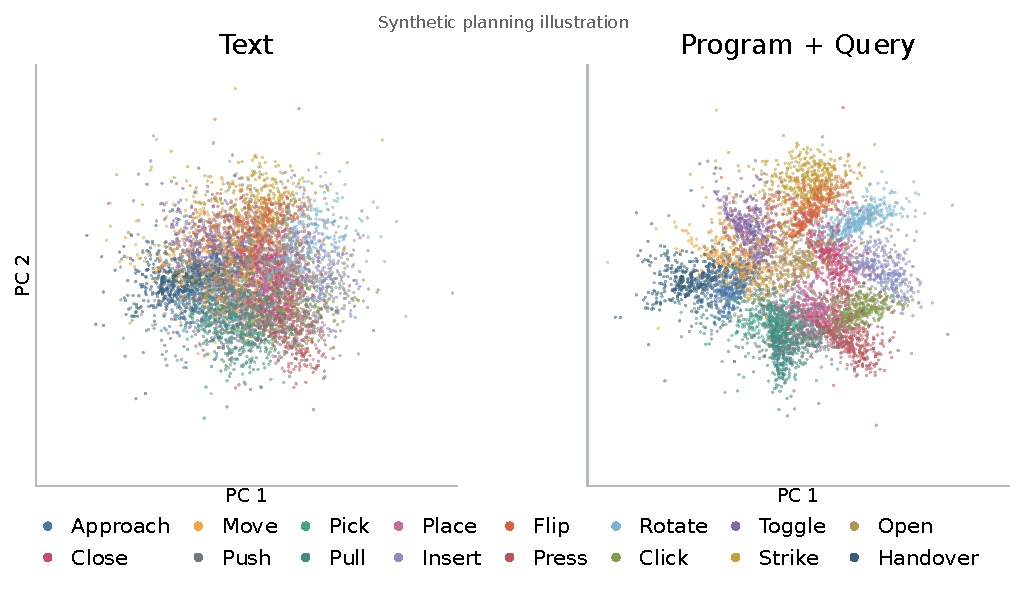
\includegraphics[width=\columnwidth]{expected_feature_comparison.pdf}
\caption{\textbf{Synthetic expected features.} Text and Program+Query share a PCA projection of generated 64-D features, with 6,400 points per panel. Greater within-class consistency is an assumed scenario, not a measured finding.}
\label{fig:representation}
\end{figure}

\textbf{Expected pattern and interpretation.} The generated Program+Query clouds show stronger within-class consistency while related actions can still overlap. That pattern is imposed by the generator and therefore supplies no empirical evidence. In measured features, reduced within-class distance and stronger cross-context retrieval would support the representation hypothesis only when accompanied by useful pose prediction and task performance. Compact clusters by themselves could reflect verb labels rather than better control.

\subsection{Real-Robot Tasks}
\label{sec:realrobot}
\textbf{Task suite.} Five proposed dual-arm tasks differ from the selected RoboTwin routines. \emph{Drawer stowing}: one arm braces the cabinet while the other opens the drawer, picks a utensil from the tabletop, stores it, and closes the drawer; success requires the utensil inside and a final gap $\leq5$\,mm. \emph{Peg assembly}: one arm holds a movable fixture while the other reorients a peg and inserts it into the indicated hole to a depth $\geq15$\,mm. \emph{Towel folding}: both arms grasp two marked corners, lift and fold a $40\!\times\!40$\,cm cloth across its midline, and release it with corner error $\leq3$\,cm. \emph{Surface wiping}: one arm stabilizes a board while the other picks a sponge and wipes a $10\!\times\!10$\,cm region, removing $\geq90\%$ of the marker mask. \emph{Cable plugging}: one arm holds a keyed socket while the other picks a loose cabled connector, aligns its key, and inserts it with a final seating gap $\leq2$\,mm.

\textbf{Purpose and procedure.} We test program composition, geometric grounding, and planner--controller feedback under articulation, precise contact, deformation, and sustained contact. Each method receives matched demonstrations and 30 planned trials per task on shared initial layouts, with randomized object pose and method order. Table~\ref{tab:realrobot} compares planner+$\pi_{0.5}$, text conditioning, and AtomVLA with feedback off/on. Success requires every task stage; timeouts, human assistance, and safety stops count as failures. Proposed hardware-independent dimensions, randomization ranges, time limits, and outcome measurements are in Appendix~\ref{app:realrobot}; hardware-specific calibration remains to be finalized.

\begin{strip}
\begin{minipage}{\textwidth}
\captionsetup{type=table}
\centering\small
\setlength{\tabcolsep}{5pt}
\caption{\textbf{Five real-robot tasks: projected success (\%).} Rows are controller variants and columns are physical tasks. All entries are planning estimates, not physical measurements.}
\label{tab:realrobot}
\begin{tabularx}{\textwidth}{@{}p{43mm}*{5}{>{\centering\arraybackslash}X}@{}}
\toprule
Method & \shortstack{Drawer stowing} & \shortstack{Peg assembly} & \shortstack{Towel folding} & \shortstack{Surface wiping} & \shortstack{Cable plugging}\\
\midrule
Planner + $\pi_{0.5}$ & 42.3 & 31.8 & 24.6 & 58.7 & 28.4\\
Planner + text-loss & 50.7 & 37.4 & 33.1 & 64.2 & 35.7\\
\model{} (feedback off) & 64.1 & 52.7 & 45.8 & 74.6 & 49.2\\
\model{} (feedback on) & 70.6 & 61.3 & 52.4 & 80.9 & 57.8\\
\bottomrule
\end{tabularx}
\end{minipage}
\end{strip}

\textbf{Expected results and interpretation.} The projected mean is 64.6\% with feedback, versus 57.3\% without it and 44.2\% for text-loss control. Folding and plugging remain harder than wiping, reflecting deformation and precise contact constraints that an endpoint pose alone cannot resolve. If the planned paired trials reproduce gains across these different task families, they would support physical transfer and feedback utility beyond the selected simulator routines. A gain confined to one task would justify a narrower conclusion; measured failures and annotation cost must accompany the success rates.

\FloatBarrier
